\section{Langkah-Langkah Percobaan} 
\subsection{Wireless Point to Point}
\begin{enumerate}
    \item Kabel LAN disambungkan dari laptop ke router pertama, lalu dilanjutkan dari router tersebut ke router lainnya.
    \item Proses login dilakukan melalui identifikasi MAC address, kemudian router di-reset ke konfigurasi default menggunakan aplikasi Winbox sebelum dilakukan pengaturan ulang.
    \begin{figure}[H]
        \centering
        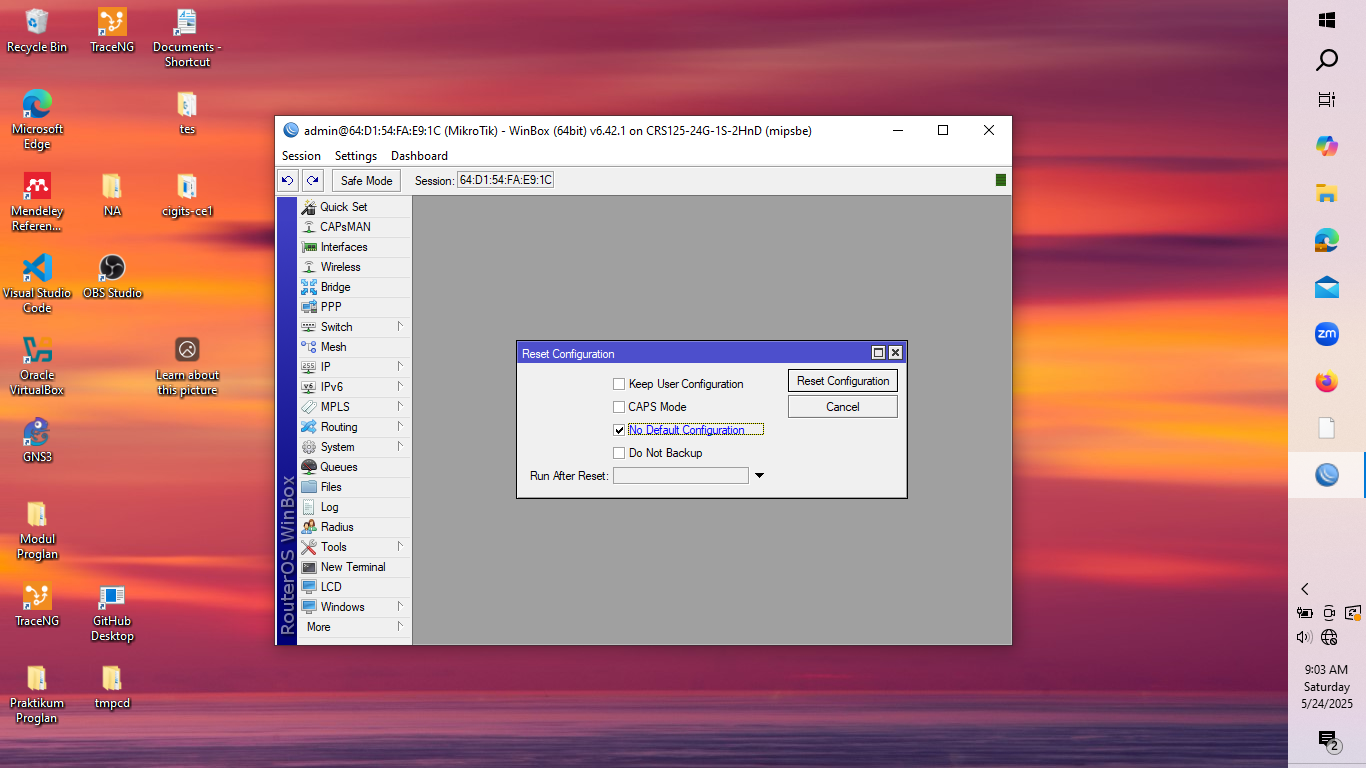
\includegraphics[width=0.5\linewidth]{P3/img/gambar1.png}
        \caption{Melakukan reset konfigurasi router melalui Winbox}
        \label{fig:reset-router}
    \end{figure}

    \item Aktifkan antarmuka nirkabel wlan1 dengan mengakses menu Wireless > WiFi Interfaces, lalu pilih wlan1 dan klik ikon panah biru untuk mengaktifkannya. Setelah itu, ubah mode menjadi bridge dan atur SSID ke \texttt{PointToPoint\_16}.

    \item Pada Router B, aktifkan antarmuka wlan1, kemudian ubah mode operasinya menjadi station agar dapat terhubung ke jaringan nirkabel yang telah disiapkan.
    \begin{figure}[H]
        \centering
        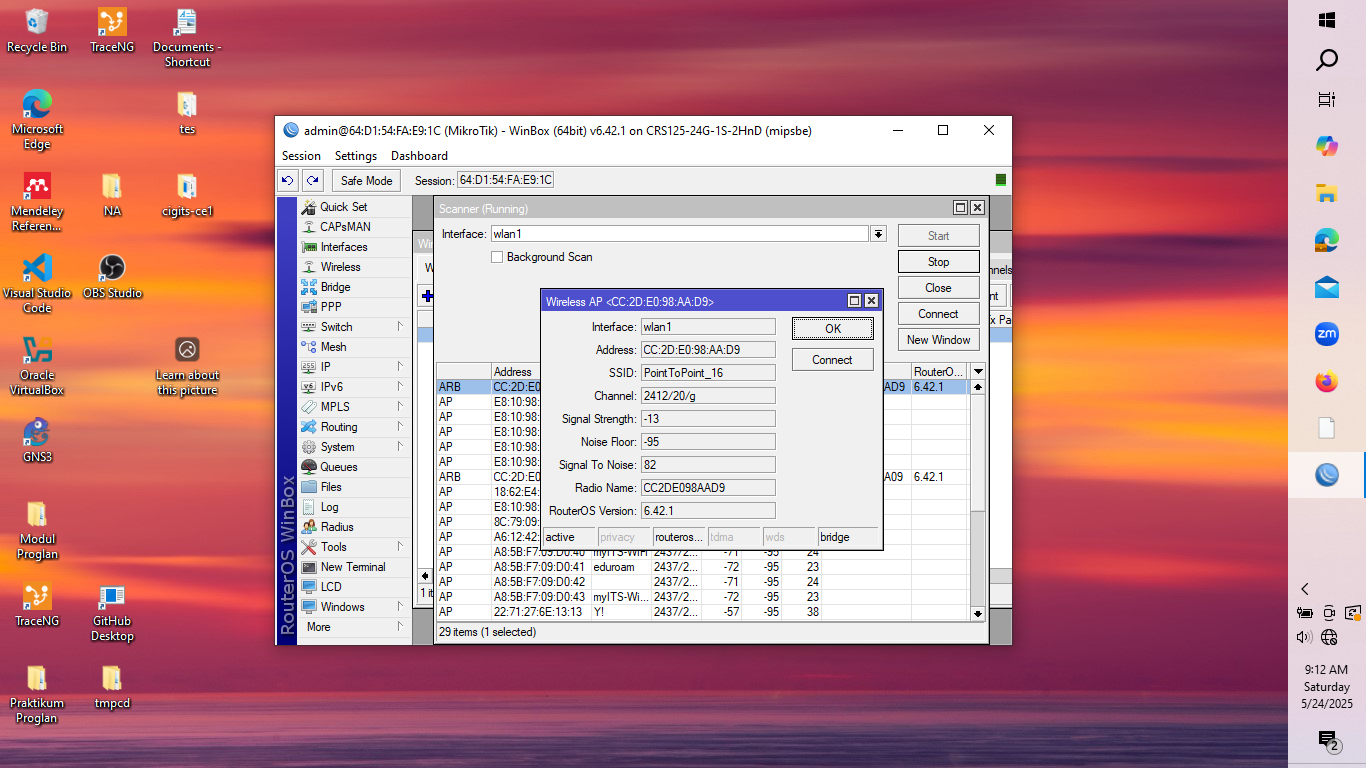
\includegraphics[width=0.5\linewidth]{P3/img/gambar3.png}
        \caption{Aktivasi Interface Wireless pada Router B}
        \label{fig:aktif-wlan-b}
    \end{figure}

    \item Di Laptop B, tekan tombol Scan, pilih jaringan dengan SSID \texttt{PointToPoint\_16}, kemudian klik Connect untuk menghubungkan.
    \begin{figure}[H]
        \centering
        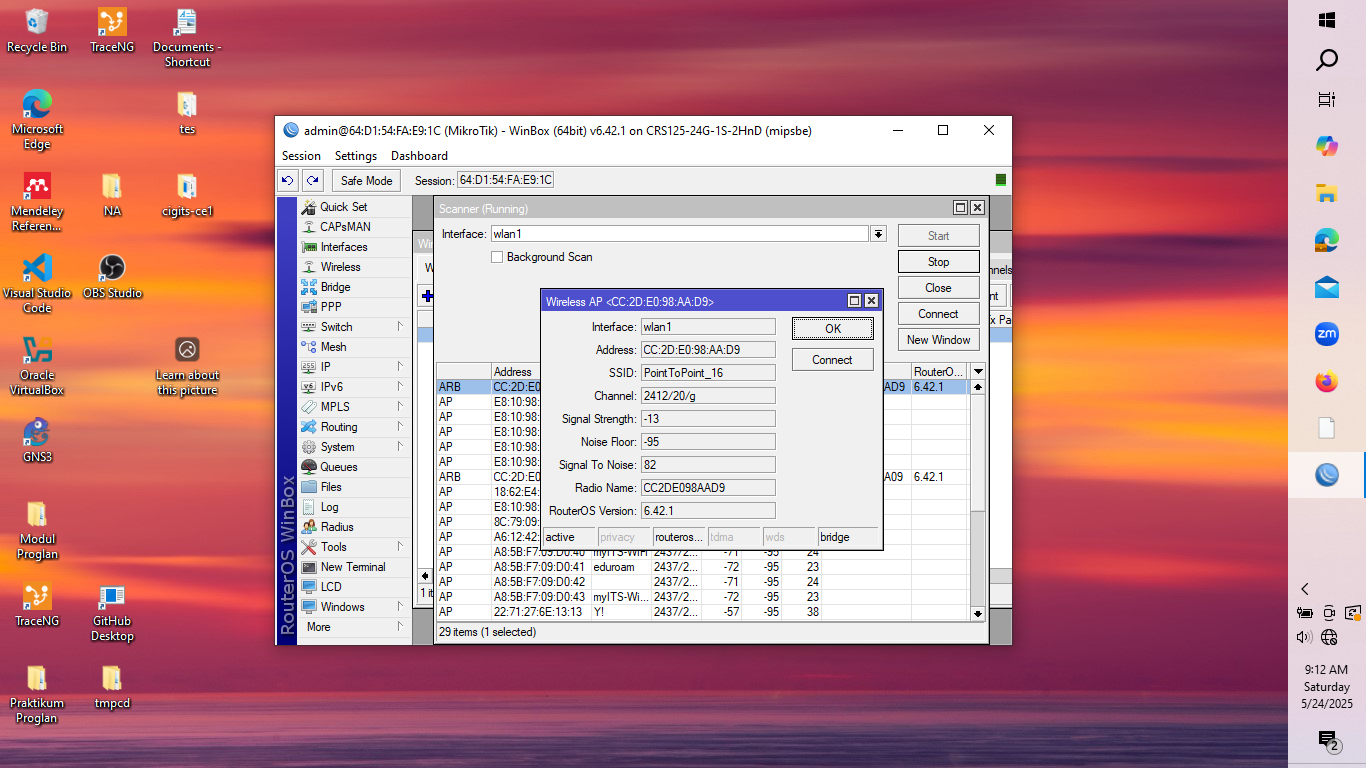
\includegraphics[width=0.5\linewidth]{P3/img/gambar3.png}
        \caption{Menghubungkan Laptop B dengan Router A melalui Jaringan Wireless}
        \label{fig:hubungkan-laptop}
        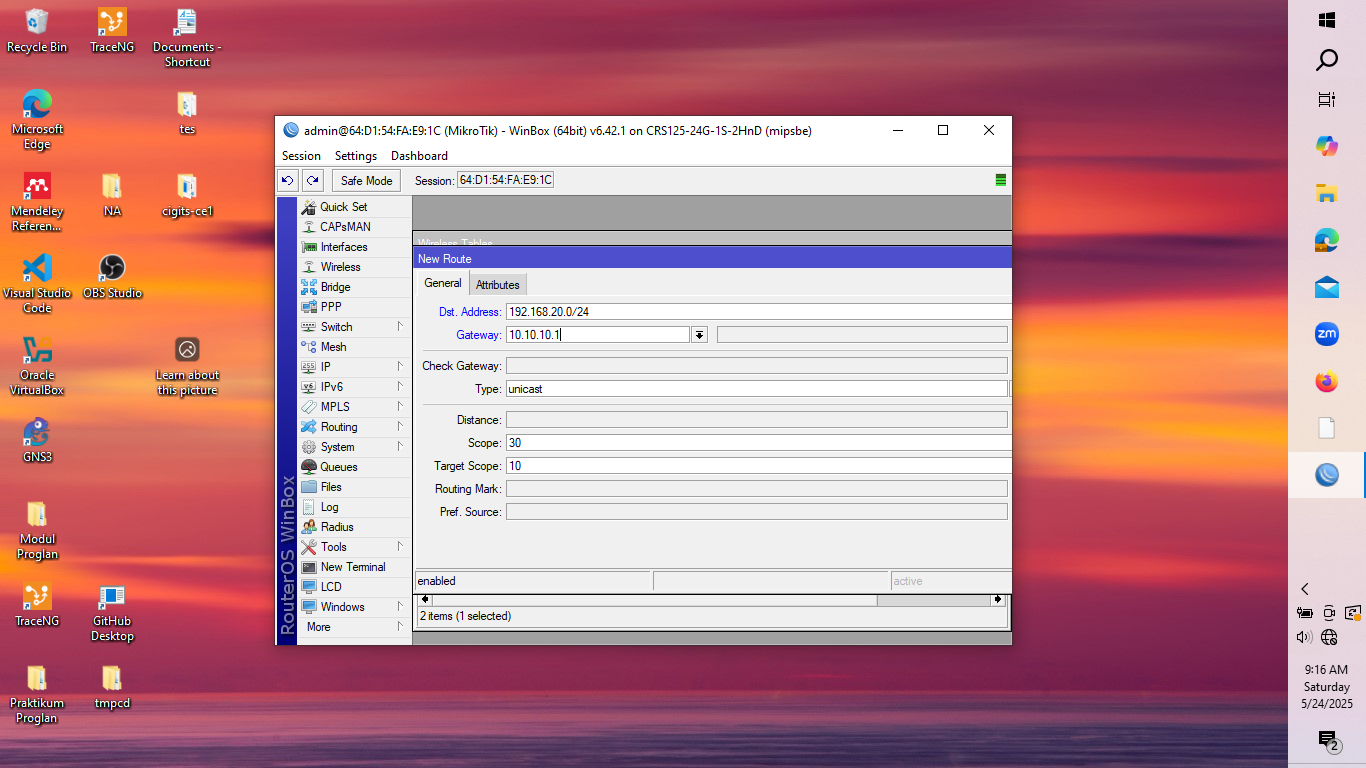
\includegraphics[width=0.5\linewidth]{P3/img/gambar5.png}
        \caption{Proses Konfigurasi IP Address di Laptop}
        \label{fig:ip-laptop}
    \end{figure}

    \item Uji konektivitas jaringan dengan melakukan perintah ping dari Laptop A ke Laptop B, serta sebaliknya.
    \begin{figure}[H]
        \centering
        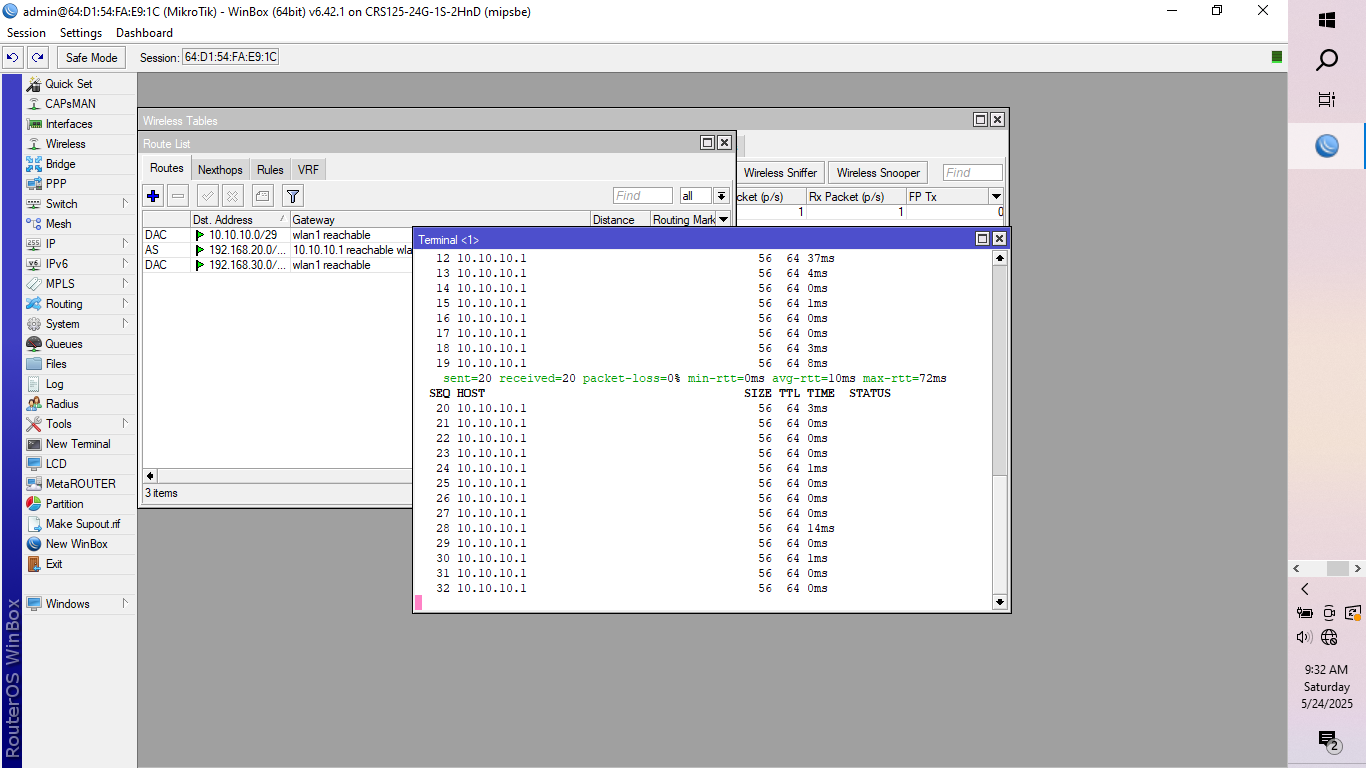
\includegraphics[width=0.5\linewidth]{P3/img/ping1.png}
        \caption{Pengujian Konektivitas: Ping Laptop A ke Laptop B}
        \label{fig:ping-ptp}
    \end{figure}
\end{enumerate}

\subsection{Wireless Point to Multipoint}
\begin{enumerate}
    \item Kabel LAN digunakan untuk menghubungkan laptop ke router, kemudian sambungan LAN dilanjutkan antar router.
    \item Proses login dilakukan dengan autentikasi berdasarkan MAC address, kemudian router di-reset menggunakan aplikasi Winbox sebelum konfigurasi ulang.
    \begin{figure}[H]
        \centering
        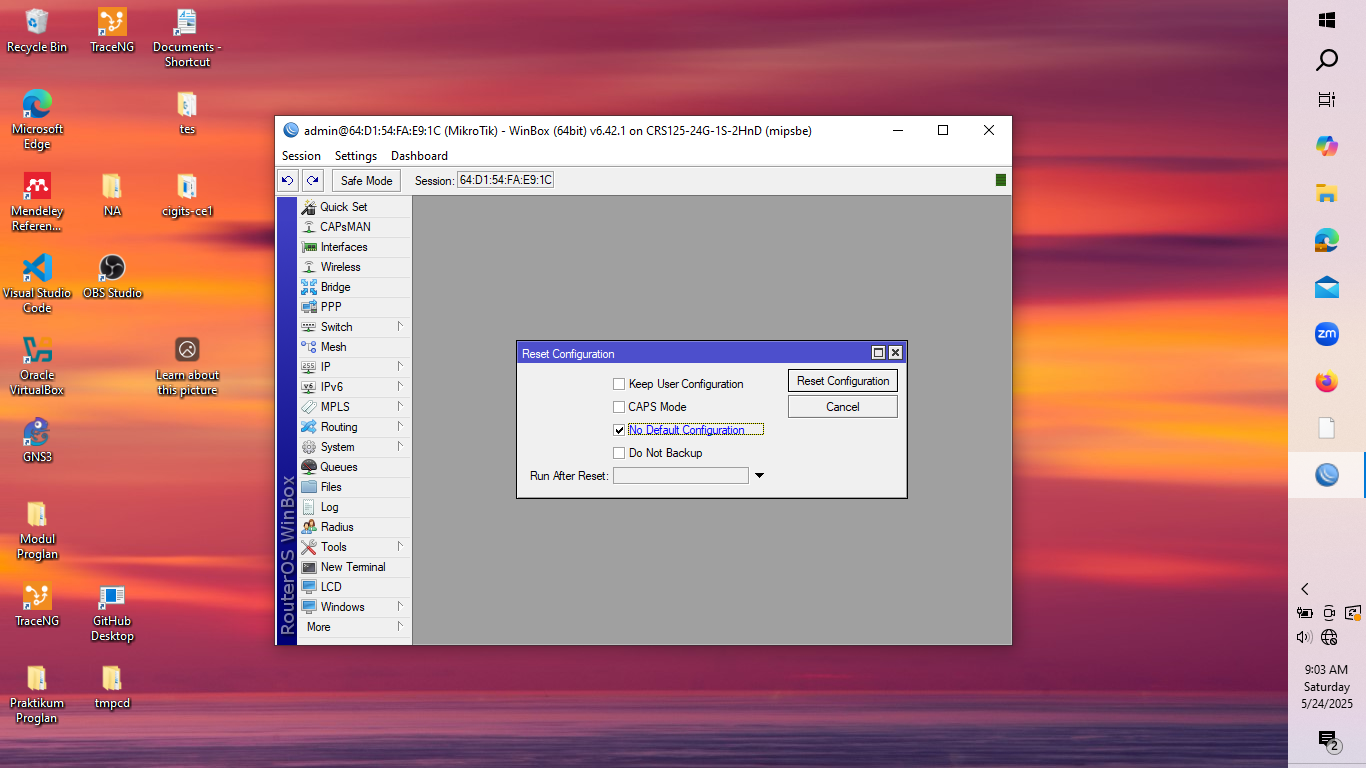
\includegraphics[width=0.5\linewidth]{P3/img/gambar1.png}
        \caption{Melakukan reset konfigurasi router melalui Winbox.}
        \label{fig:reset-router-multi}
    \end{figure}

    \item Pada Router A, aktifkan interface wlan1 dan ubah mode operasinya menjadi AP bridge dengan SSID \texttt{PointToMultiPoint\_16}.
 

    \item Pada Router B, aktifkan interface wlan1 dan ubah mode menjadi station bridge.
    \begin{figure}[H]
        \centering
        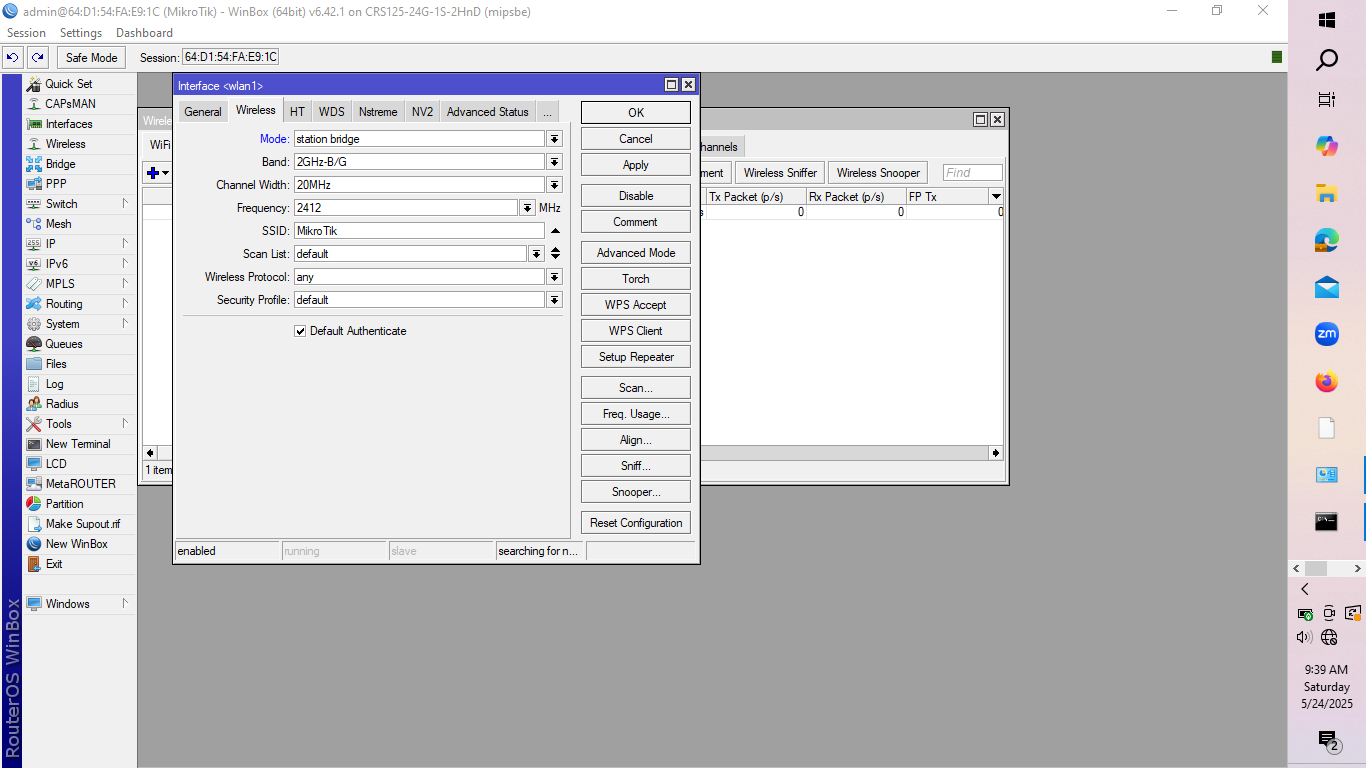
\includegraphics[width=0.5\linewidth]{P3/img/gambar3ma.png}
        \caption{Konfigurasi dan Aktivasi Wireless Interface pada Router B (Multipoint Setup)}
        \label{fig:aktif-wlan-b-multi}
    \end{figure}

    \item Di Laptop B, tekan tombol Scan, pilih jaringan dengan SSID \texttt{PointToMultiPoint\_16}, kemudian klik Connect untuk menghubungkan.
    \begin{figure}[H]
        \centering
        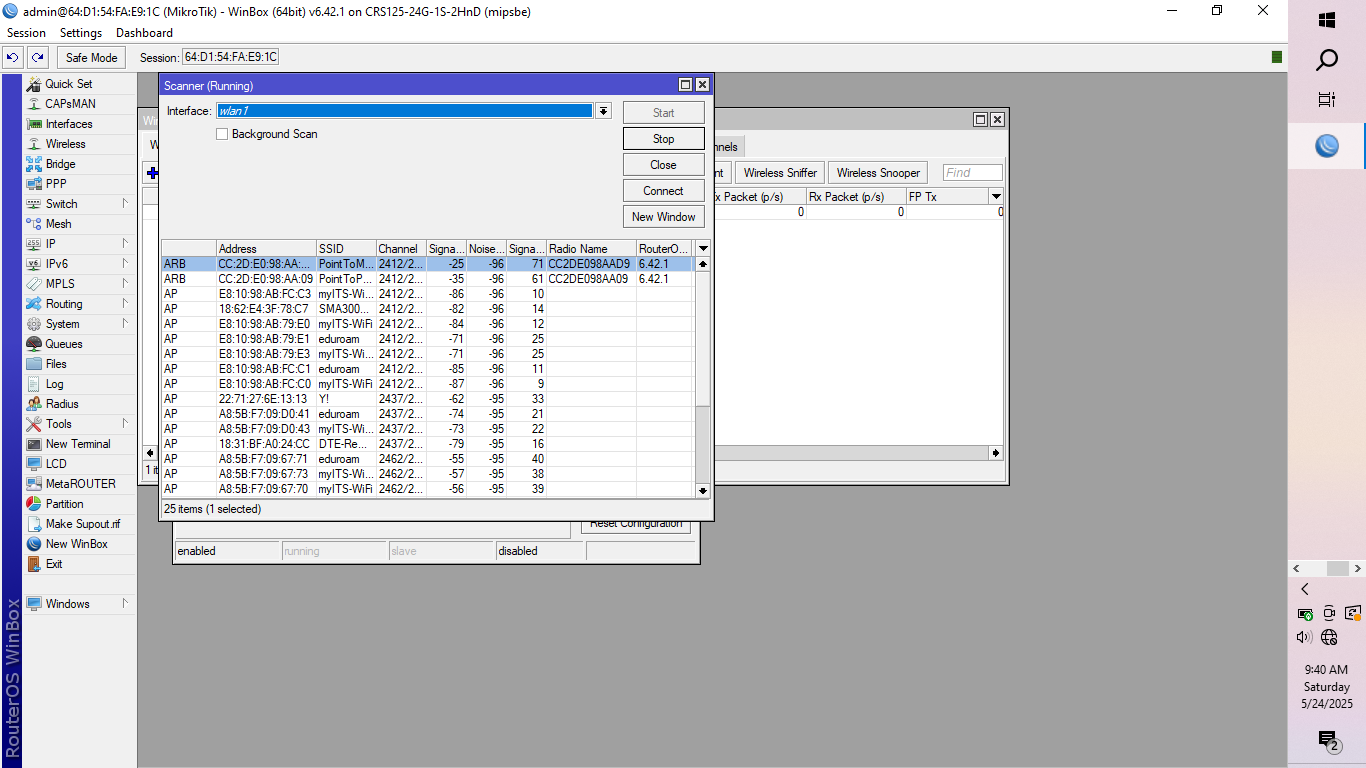
\includegraphics[width=0.5\linewidth]{P3/img/gambar3m.png}
        \caption{Proses Koneksi Laptop B ke Router A dalam Konfigurasi Multipoint}
        \label{fig:hubungkan-laptop-multi}
    \end{figure}

    \item Lakukan konfigurasi alamat IP pada interface WLAN dan ether2 di kedua router.
    \begin{figure}[H]
        \centering
        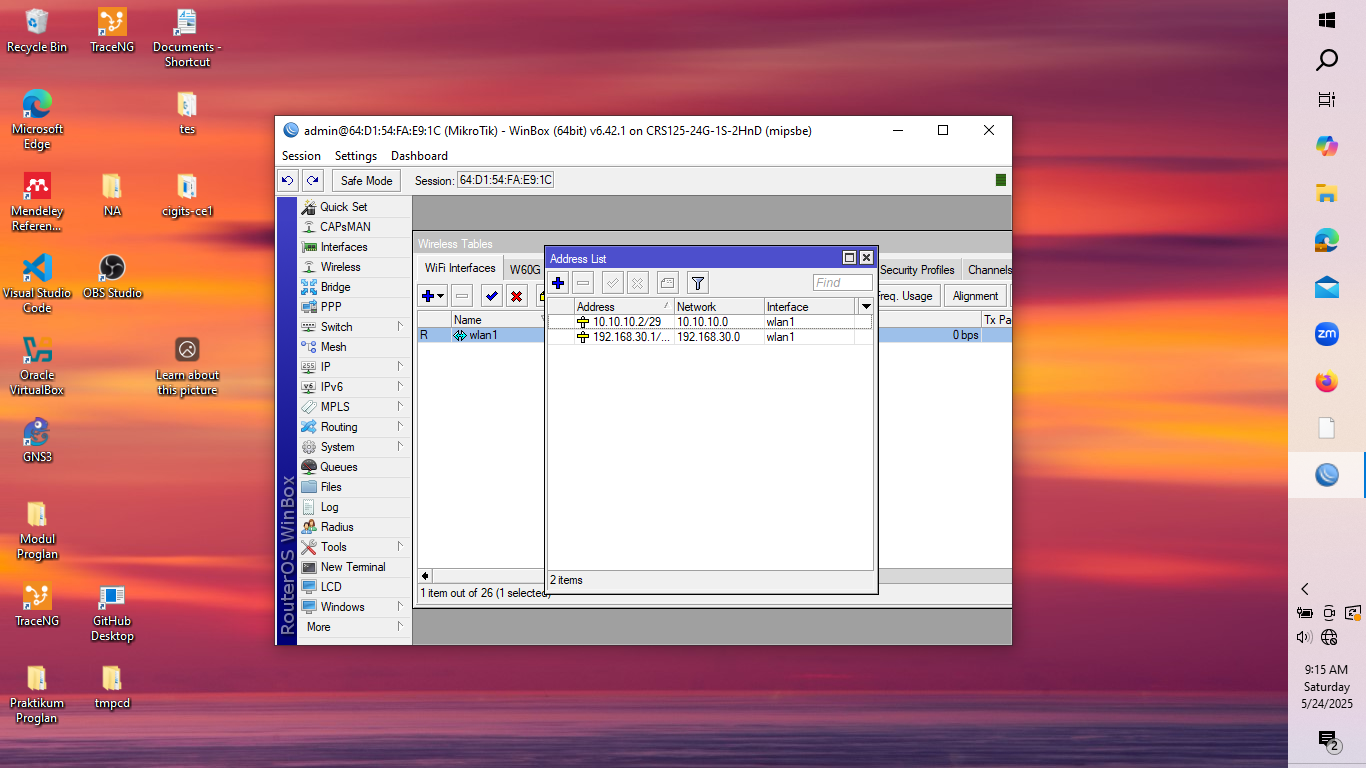
\includegraphics[width=0.5\linewidth]{P3/img/gambar4.png}
        \caption{Pengaturan Alamat IP pada Router A dan B dalam Jaringan Multipoint}
        \label{fig:ip-router-multi}
    \end{figure}

    \item Lakukan penambahan routing statis pada perangkat jaringan.
    \begin{figure}[H]
        \centering
        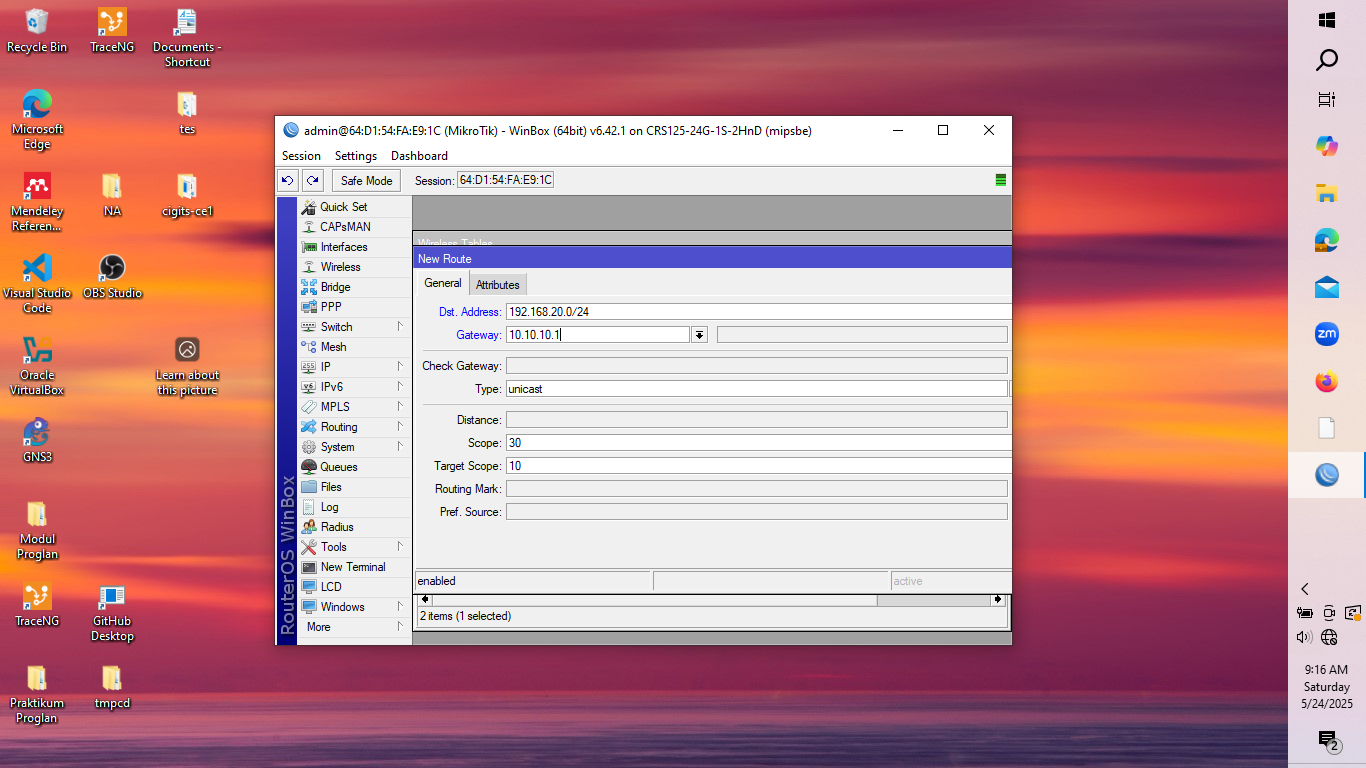
\includegraphics[width=0.5\linewidth]{P3/img/gambar5.png}
        \caption{Konfigurasi Penambahan Routing Statis pada Router A dan B dalam Jaringan Multipoint}
        \label{fig:routing-multi}
    \end{figure}

    \item Lakukan konfigurasi alamat IP pada laptop dengan mengakses pengaturan jaringan di Control Panel.
    \begin{figure}[H]
        \centering
        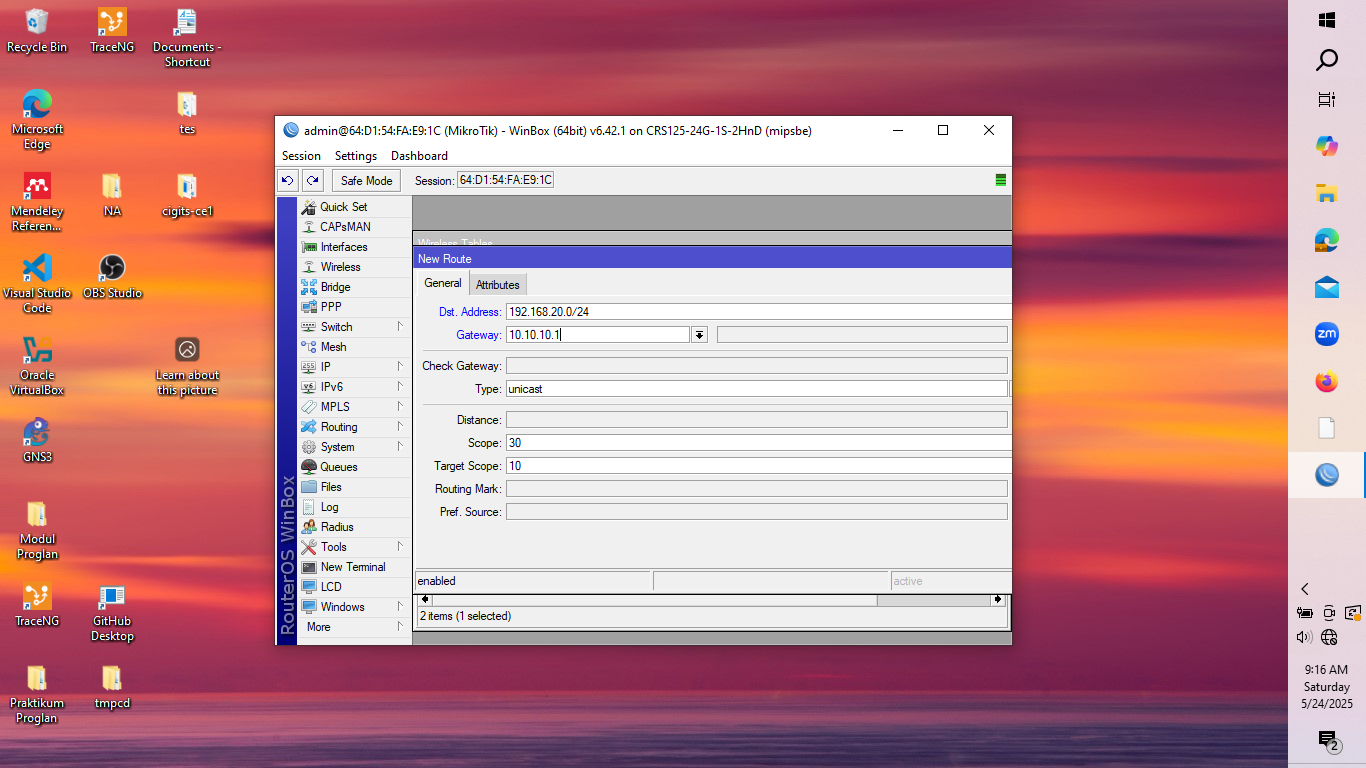
\includegraphics[width=0.5\linewidth]{P3/img/gambar5.png}
        \caption{Pengaturan Alamat IP pada Laptop untuk Jaringan Multipoint}
        \label{fig:ip-laptop-multi}
    \end{figure}

    \item Lakukan pengujian konektivitas jaringan dengan perintah ping dari Laptop A ke Laptop B.
    \begin{figure}[H]
        \centering
        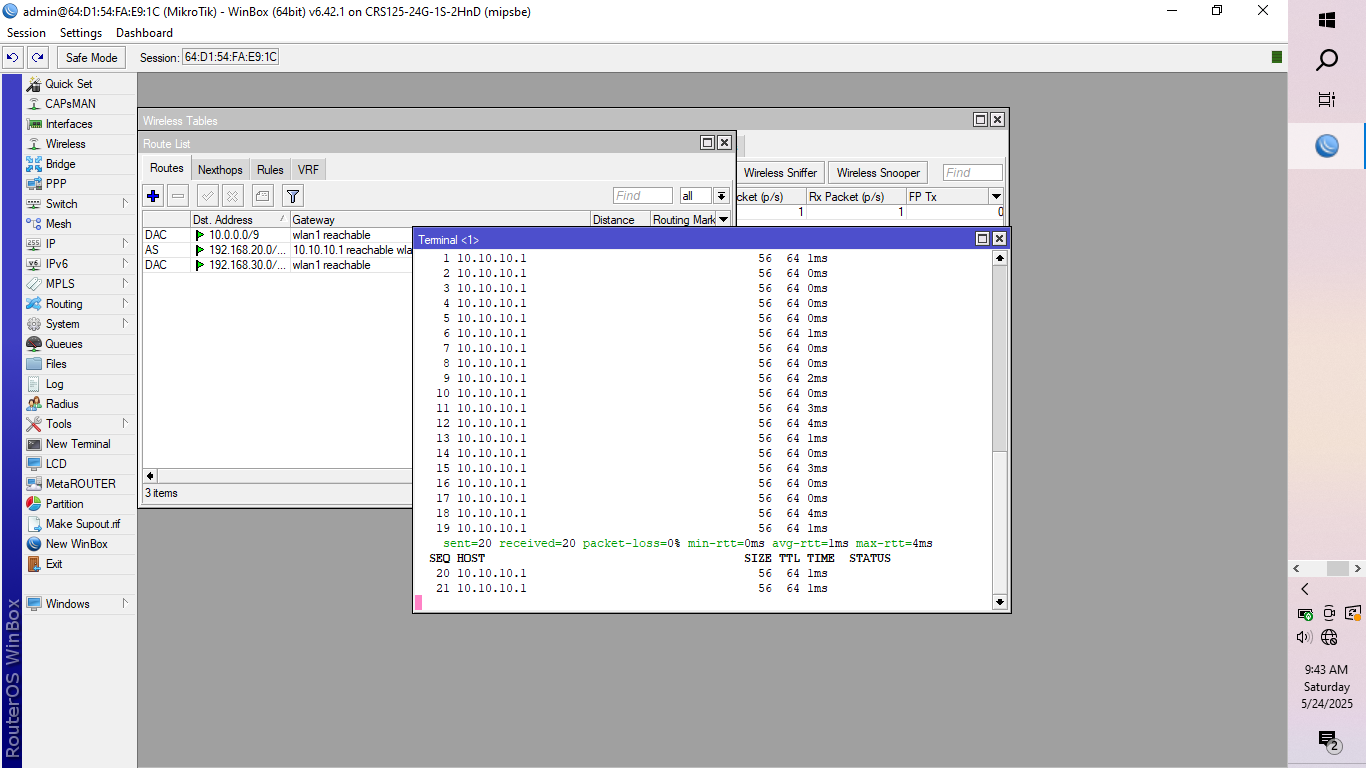
\includegraphics[width=0.5\linewidth]{P3/img/ping2.png}
        \caption{Uji koneksi ping Laptop A ke Laptop B (Multipoint).}
        \label{fig:ping-multi}
    \end{figure}
\end{enumerate}

\subsection{Wireless Bridge}
\begin{enumerate}
    \item Kabel LAN digunakan untuk menghubungkan laptop ke router, kemudian sambungan LAN diteruskan antar router.
    \item Proses login dilakukan dengan autentikasi berdasarkan MAC address, kemudian router di-reset menggunakan aplikasi Winbox sebelum konfigurasi ulang.
    \begin{figure}[H]
        \centering
        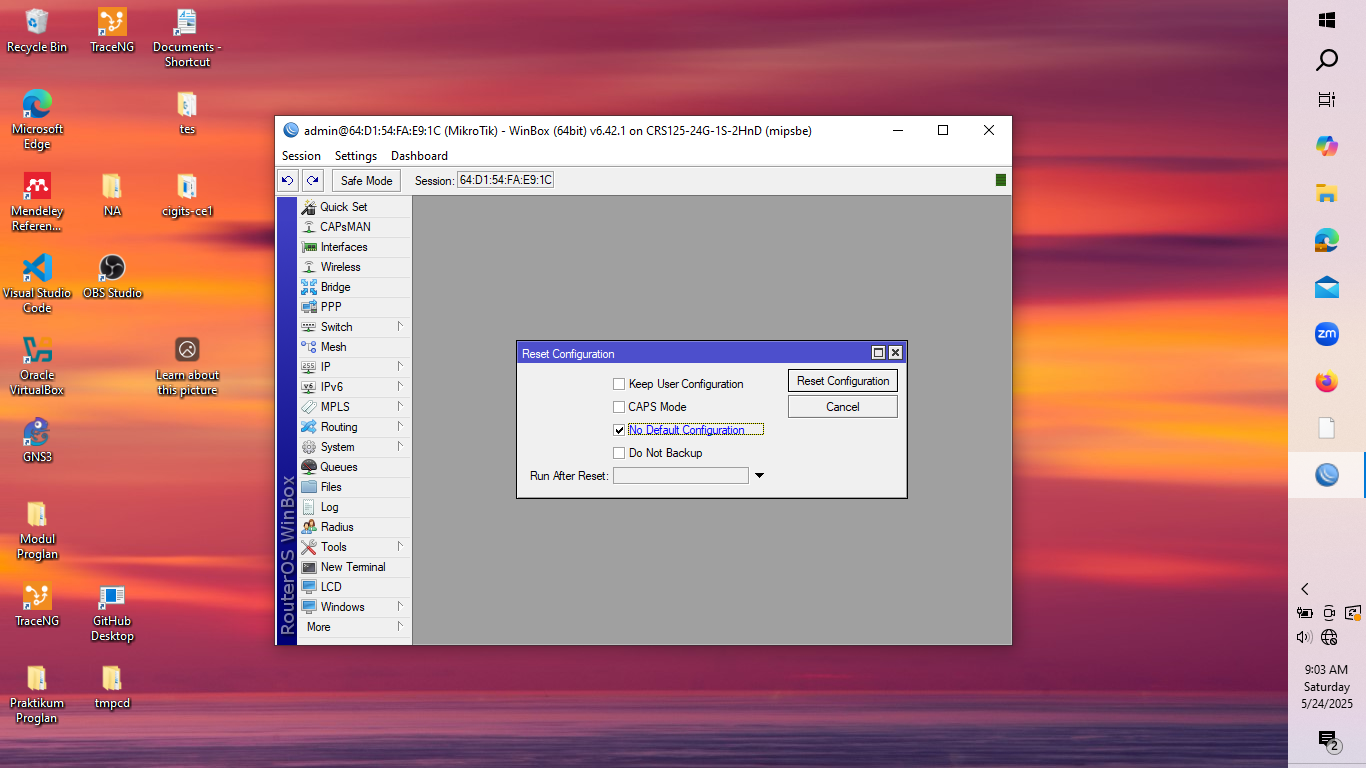
\includegraphics[width=0.5\linewidth]{P3/img/gambar1.png}
        \caption{Melakukan reset konfigurasi router melalui Winbox.}
        \label{fig:reset-bridge}
    \end{figure}

    \item Pada Router A, aktifkan interface \texttt{wlan1}, kemudian setel mode operasinya ke \textbf{bridge} dan konfigurasi SSID menjadi \texttt{WirelessBridge\_16}.

    \item Aktifkan interface \texttt{wlan1} pada Router B, lalu ubah mode menjadi \textbf{station pseudobridge}..
    \begin{figure}[H]
        \centering
        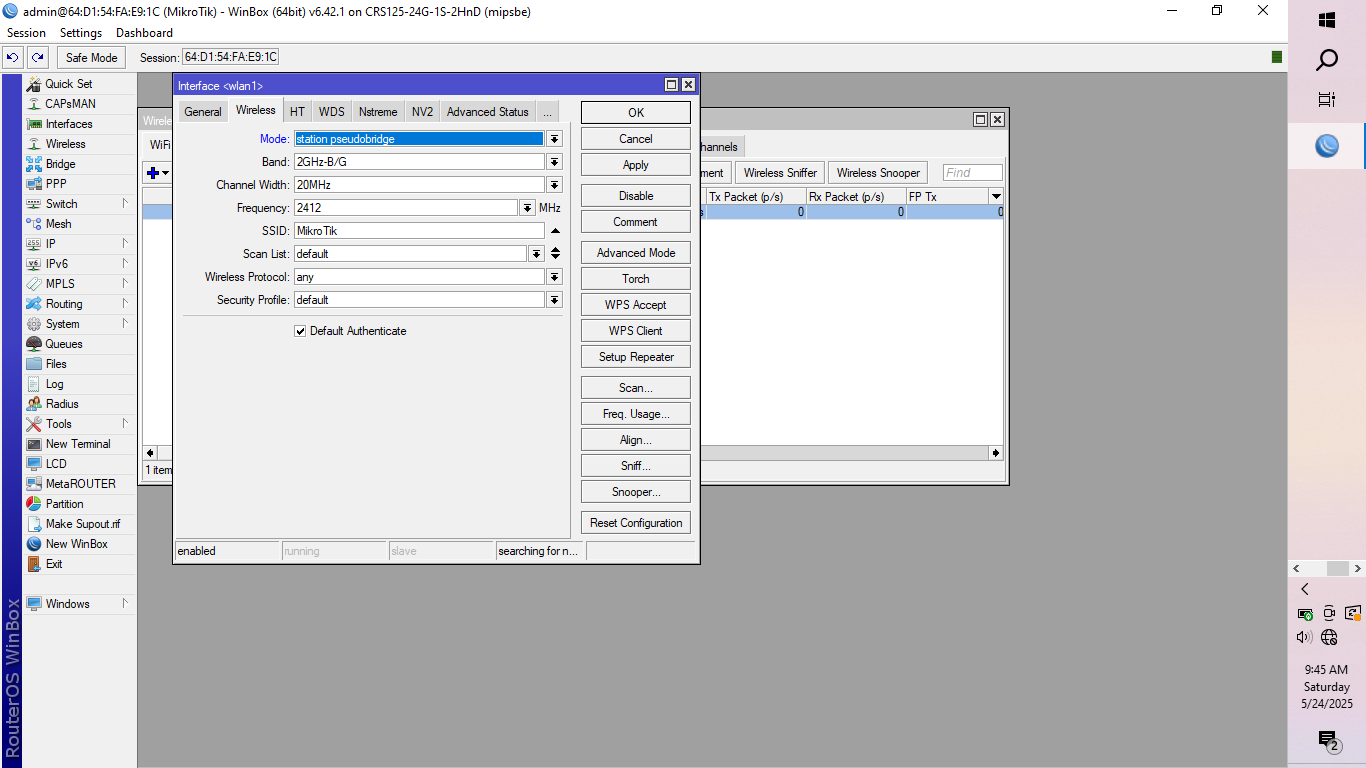
\includegraphics[width=0.5\linewidth]{P3/img/gambar3w.png}
        \caption{Mengaktifkan Interface Wireless pada Router B dalam Mode Bridge}
        \label{fig:wlan-b-bridge}
    \end{figure}

    \item Scan jaringan wireless, kemudian pilih dan hubungkan ke SSID \texttt{WirelessBridge\_16}..
    \begin{figure}[H]
        \centering
        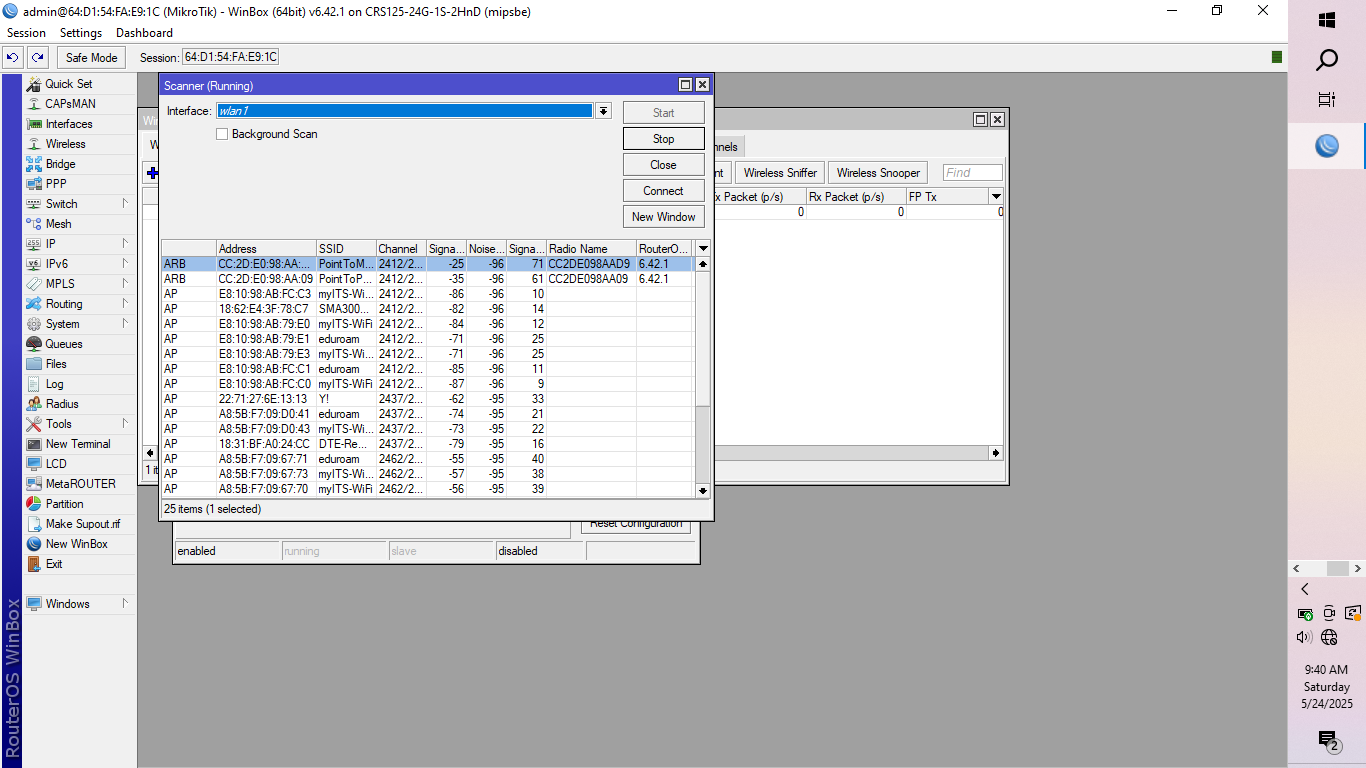
\includegraphics[width=0.5\linewidth]{P3/img/gambar3m.png}
        \caption{Menghubungkan Perangkat ke Jaringan dengan SSID Wireless Bridge}
        \label{fig:ssid-bridge}
    \end{figure}

    \item Lakukan pengaturan alamat IP pada interface wlan dan ether2.
    \begin{figure}[H]
        \centering
        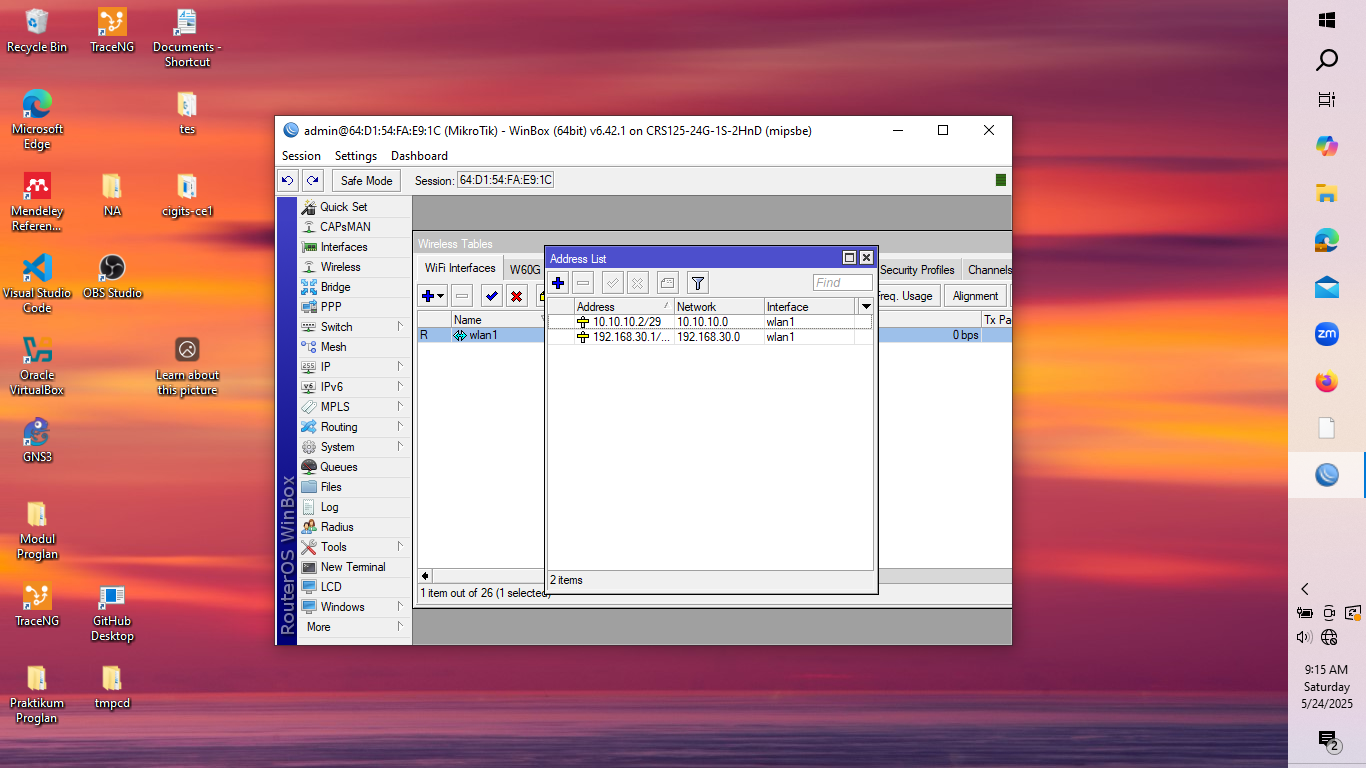
\includegraphics[width=0.5\linewidth]{P3/img/gambar4.png}
        \caption{Konfigurasi IP pada Router A dan B dalam Mode Bridge}
        \label{fig:ip-bridge}
    \end{figure}

    \item Lakukan penambahan routing statis untuk mengarahkan lalu lintas jaringan sesuai kebutuhan.
    \begin{figure}[H]
        \centering
        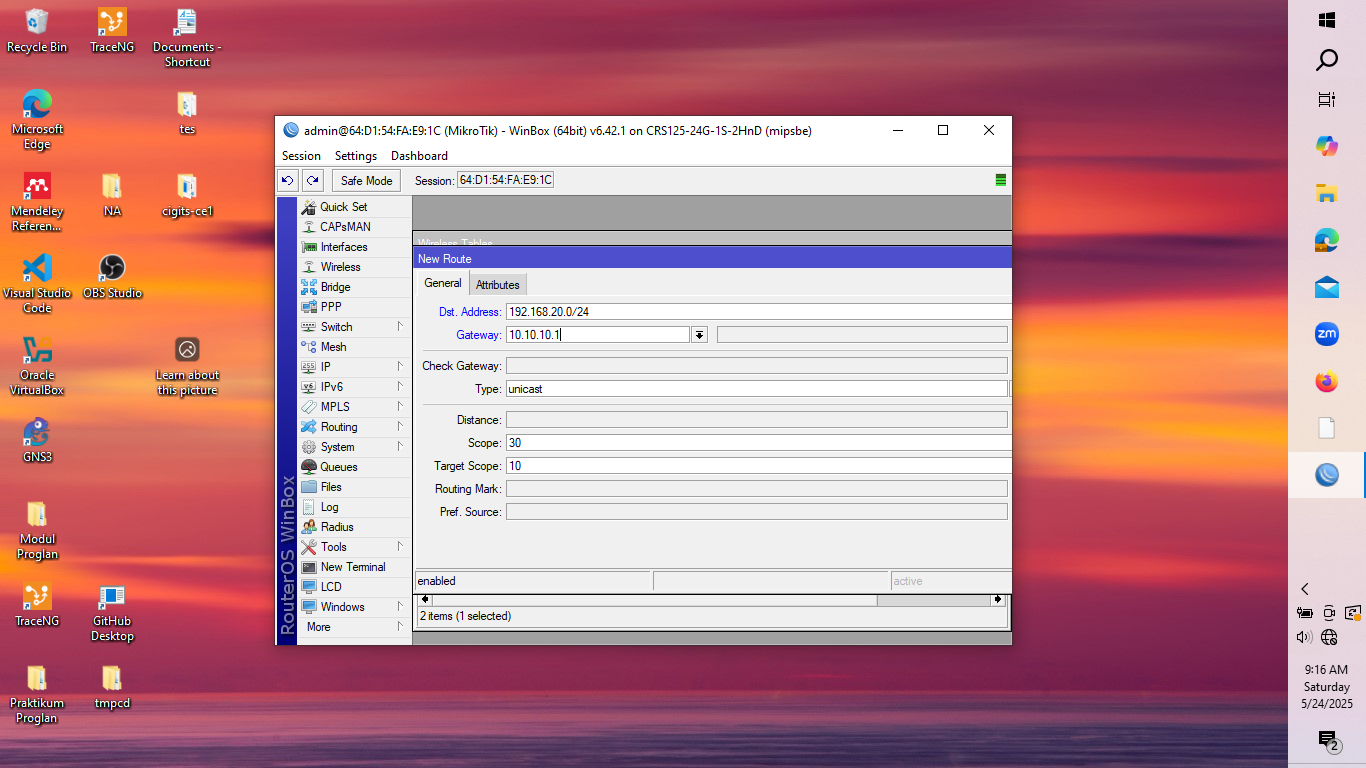
\includegraphics[width=0.5\linewidth]{P3/img/gambar5.png}
        \caption{Konfigurasi Routing Statis pada Router A dan B dalam Topologi Bridge}
        \label{fig:routing-bridge}
    \end{figure}

    \item Pengaturan Alamat IP pada Laptop
    \begin{figure}[H]
        \centering
        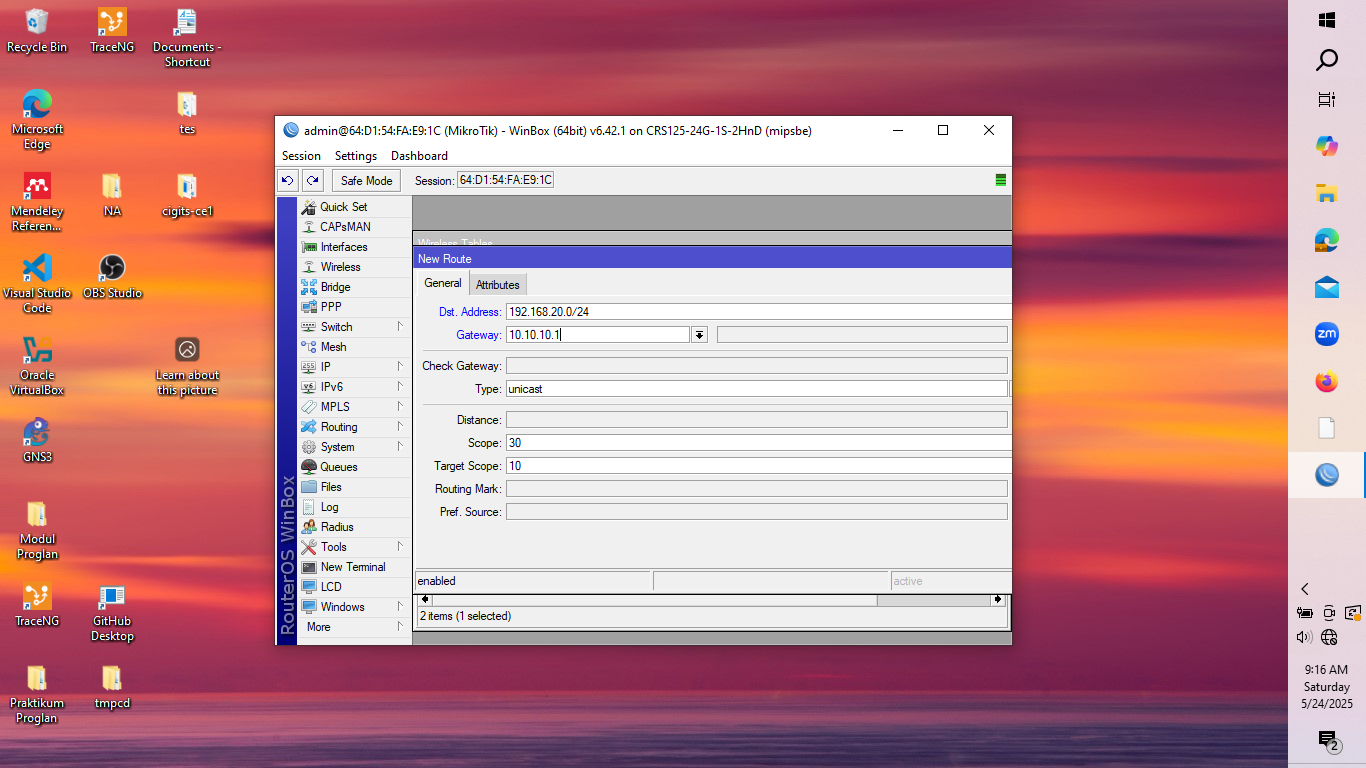
\includegraphics[width=0.5\linewidth]{P3/img/gambar5.png}
        \caption{Pengaturan Alamat IP Laptop dalam Topologi Bridge}
        \label{fig:ip-laptop-bridge}
    \end{figure}
    
    \item Uji koneksi antar perangkat dengan metode ping.
    \begin{figure}[H]
        \centering
        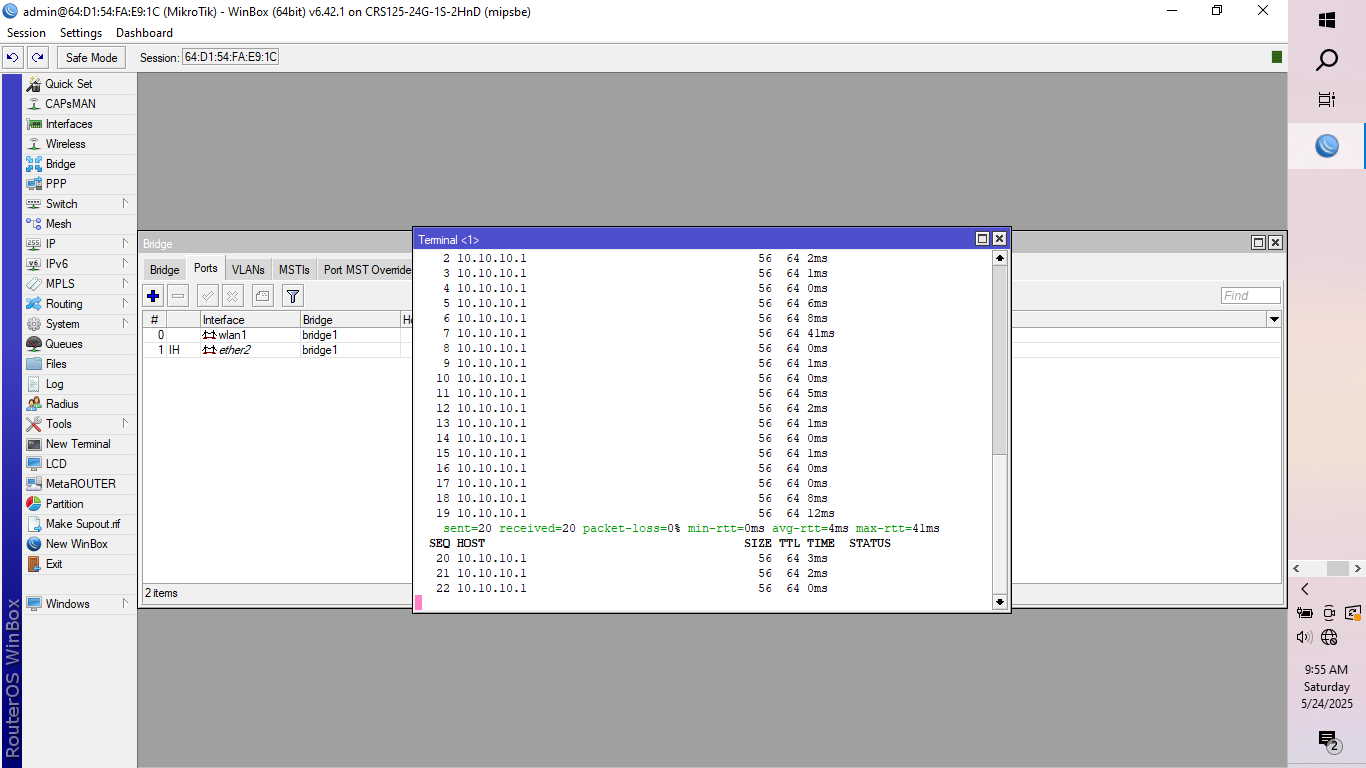
\includegraphics[width=0.5\linewidth]{P3/img/ping3.png}
        \caption{Pengujian koneksi ping antara Laptop A dan Laptop B dalam jaringan Bridge.}
        \label{fig:ping-bridge}
    \end{figure}
\end{enumerate}



\section{Analisis Hasil Percobaan}
Dalam praktikum ini, dilakukan pengujian terhadap tiga jenis konfigurasi jaringan nirkabel menggunakan perangkat router, yaitu Wireless Point to Point, Wireless Point to Multipoint, dan Wireless Bridge. Setiap topologi memiliki karakteristik, tujuan, dan hasil pengujian yang berbeda-beda.

Untuk konfigurasi Wireless Point to Point, dua router dikonfigurasi agar dapat saling berkomunikasi secara langsung. Router A diatur sebagai bridge, sementara Router B berperan sebagai station, keduanya menggunakan SSID yang sama, yaitu PointToPoint16. Setelah proses pengaturan alamat IP dan routing statis selesai, dilakukan pengujian konektivitas menggunakan perintah ping dari Laptop A ke Laptop B. Hasil pengujian menunjukkan koneksi yang stabil dengan waktu respons yang cepat dan tanpa kehilangan paket. Konfigurasi ini ideal digunakan untuk menghubungkan dua titik secara langsung dengan koneksi yang stabil serta penggunaan bandwidth yang efisien.

Pada konfigurasi Wireless Point to Multipoint, Router A difungsikan sebagai access point dalam mode bridge, dan Router B dikonfigurasi sebagai station bridge yang terhubung ke SSID PointToMultiPoint16. Topologi ini memungkinkan beberapa perangkat client untuk terhubung ke satu access point secara bersamaan. Setelah konfigurasi IP dan routing selesai, dilakukan uji koneksi dengan ping, dan hasilnya menunjukkan bahwa koneksi berhasil dilakukan. Namun, konfigurasi ini membutuhkan manajemen jaringan yang lebih rumit karena jumlah client yang bertambah dapat menurunkan performa akibat peningkatan interferensi sinyal dan pembagian bandwidth.

Sementara itu, dalam konfigurasi Wireless Bridge, fokus utama adalah menghubungkan dua jaringan LAN secara virtual menggunakan koneksi nirkabel. Router A tetap dikonfigurasi sebagai bridge, sedangkan Router B menggunakan mode station pseudobridge. Setelah koneksi berhasil dan pengaturan IP serta routing selesai, uji koneksi menggunakan ping menunjukkan komunikasi dua arah dapat dilakukan dengan baik. Namun, mode station pseudobridge memiliki keterbatasan dalam menangani lalu lintas broadcast dan multicast. Oleh karena itu, topologi ini lebih sesuai untuk jaringan berskala kecil atau skenario khusus yang membutuhkan penggabungan jaringan pada level lapisan 2 (layer 2 bridging).

\section{Hasil Tugas Modul}

    \begin{figure}[H]
        \centering
        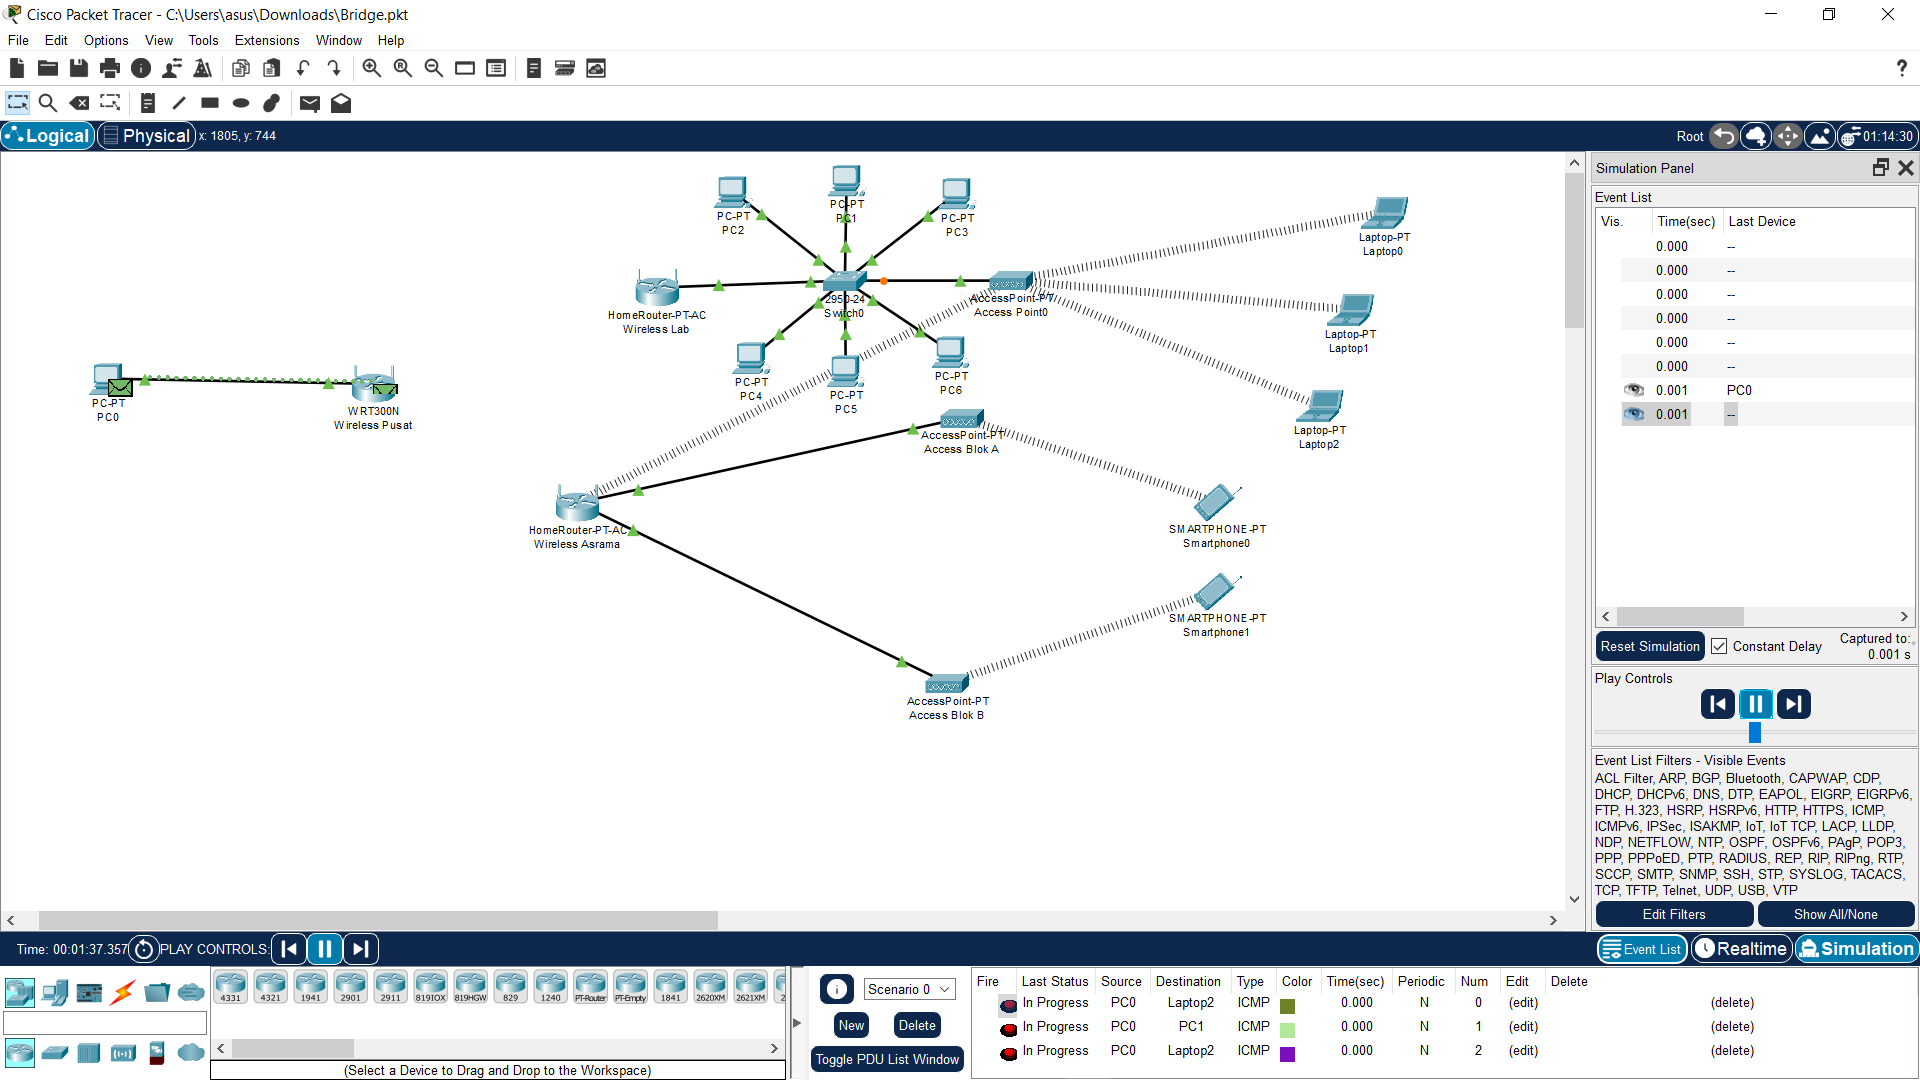
\includegraphics[width=0.5\linewidth]{P3/img/topologi.png}
        \caption{Topologi Jaringan}
        \label{fig:ping-bridge}
    \end{figure}
    
Topologi terdiri dari beberapa perangkat jaringan, baik wired maupun wireless, yang menghubungkan tiga gedung utama: Gedung Pusat, Gedung Lab, dan Gedung Asrama. Berikut deskripsi per gedung:

\subsection*{1. Gedung Pusat}
\begin{itemize}
    \item Terdapat perangkat \textbf{PC0} dan \textbf{WRt300N} (Wireless Router).
    \item Berfungsi sebagai titik pusat koneksi Point-to-Multipoint (PTMP).
\end{itemize}

\subsection*{2. Gedung Lab}
\begin{itemize}
    \item Menggunakan perangkat \textbf{HomeRouter-PT-AC} (Wireless Lab).
    \item Terhubung ke switch yang menghubungkan perangkat \textbf{PC2–PC6} dan server.
    \item Terhubung secara wireless ke jaringan utama melalui PTMP.
\end{itemize}

\subsection*{3. Gedung Asrama}
\begin{itemize}
    \item Terdiri dari dua bagian: \textbf{Blok A} dan \textbf{Blok B}.
    \item Masing-masing menggunakan \textbf{Access Point} bernama \textbf{Access Blok A} dan \textbf{Access Blok B}.
    \item Koneksi antara keduanya menggunakan \textbf{Point-to-Point (PTP) wireless bridge}.
\end{itemize}

\section*{Jenis Koneksi}
\begin{itemize}
    \item \textbf{Point-to-Multipoint (PTMP)} digunakan untuk menghubungkan Gedung Pusat dengan Gedung Lab dan Gedung Asrama.
    \item \textbf{Point-to-Point (PTP)} digunakan untuk menghubungkan Blok A dan Blok B di Gedung Asrama.
\end{itemize}

\section*{Hasil Simulasi}
\begin{itemize}
    \item Dilakukan uji konektivitas menggunakan ICMP (Ping) dari \textbf{PC0} ke \textbf{Laptop2}.
    \item Hasil menunjukkan bahwa semua jaringan wireless antar gedung dapat saling berkomunikasi dengan baik.
\end{itemize}

Simulasi jaringan berhasil dilakukan sesuai dengan permintaan soal. Koneksi wireless antar gedung menggunakan PTMP dan koneksi internal antar blok di Gedung Asrama menggunakan PTP berhasil dibangun dan diuji konektivitasnya.

\section{Kesimpulan}
Berdasarkan hasil uji coba, dapat disimpulkan bahwa setiap jenis konfigurasi jaringan nirkabel memiliki ciri khas dan kelebihan tersendiri. Konfigurasi Point to Point menunjukkan kestabilan dan efisiensi tertinggi dalam komunikasi antara dua perangkat secara langsung. Sementara itu, konfigurasi Point to Multipoint menawarkan kemudahan dalam menghubungkan banyak client, meskipun diperlukan perhatian khusus terhadap pengelolaan bandwidth dan potensi interferensi sinyal. Di sisi lain, konfigurasi Wireless Bridge memungkinkan penggabungan dua jaringan LAN secara virtual, namun kinerjanya bisa terpengaruh oleh penggunaan mode pseudobridge. Oleh karena itu, pemilihan topologi jaringan sebaiknya disesuaikan dengan kebutuhan komunikasi, jumlah perangkat yang akan digunakan, serta cakupan jaringan yang direncanakan.

\section{Lampiran}
\subsection{Dokumentasi saat praktikum}
    \begin{figure}[H]
        \centering
        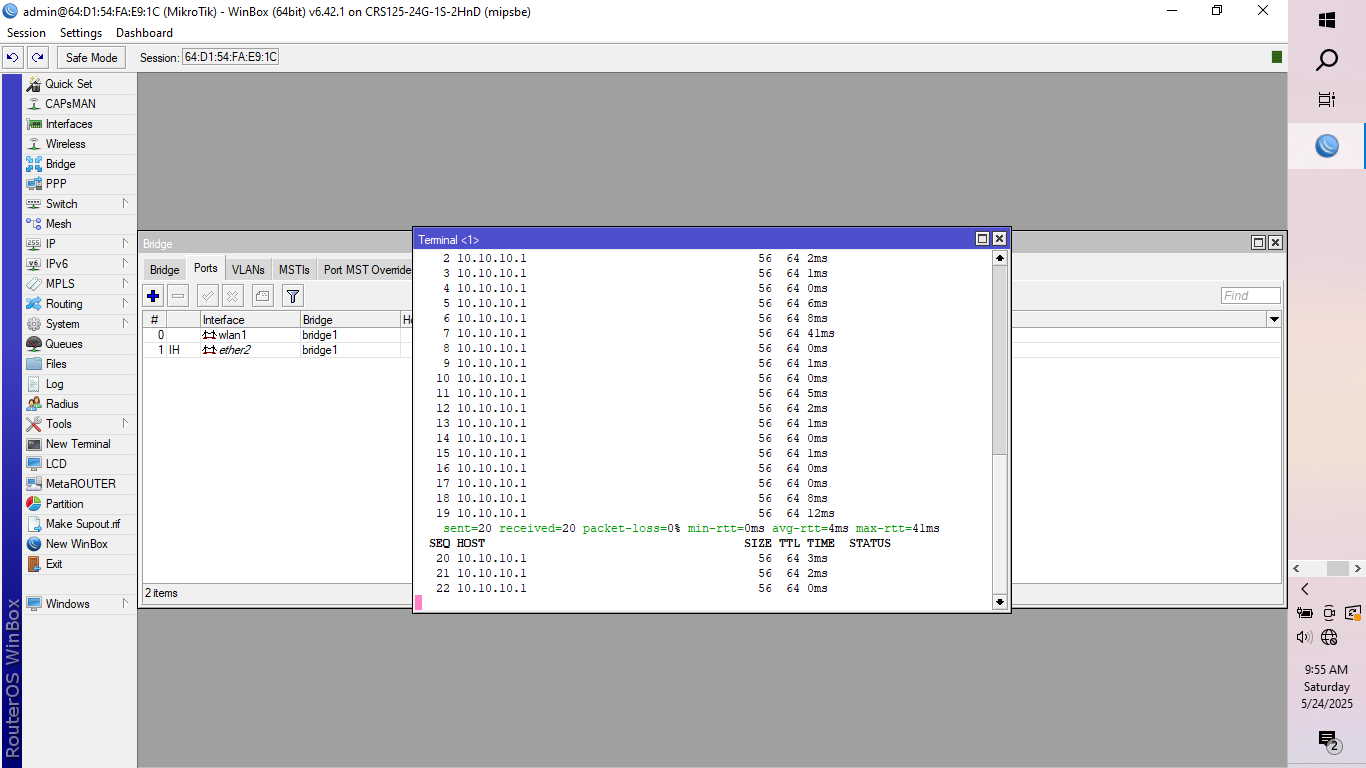
\includegraphics[width=0.5\linewidth]{P3/img/ping3.png}
        \caption{Uji koneksi (ping) antara Laptop A dan Laptop B melalui konfigurasi Bridge.}
        \label{fig:ping-bridge}
    \end{figure}

